\subsection{Level3.2: パラメータと収束能力の関連性について}
学習と各パラメータの影響について,それぞれのパラメータを変更しながらその平均値をグラフにして観察した.
\subsection{結果:HIDDEN}
\begin{figure}[h]
 \begin{center}
  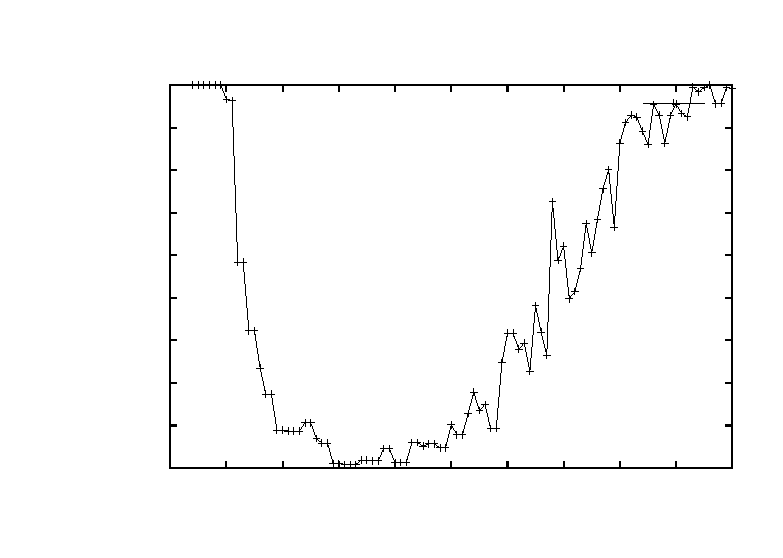
\includegraphics[width=10.0cm]{lebel3/HIDDEN.eps}
  \caption{HIDDENの増加に伴う推移}
  \label{hidden}
 \end{center}
\end{figure} 

\subsection{結果:ETA}
\begin{figure}[h]
 \begin{center}
  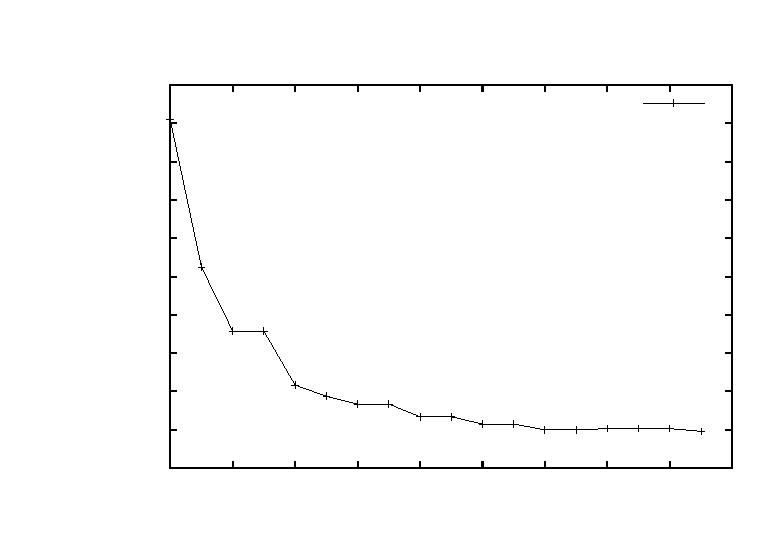
\includegraphics[width=10.0cm]{lebel3/ETA.eps}
  \caption{ETAの増加に伴う推移}
  \label{eta}
 \end{center}
\end{figure} 
	
\subsection{結果:ALPHA}
\begin{figure}[h]
 \begin{center}
  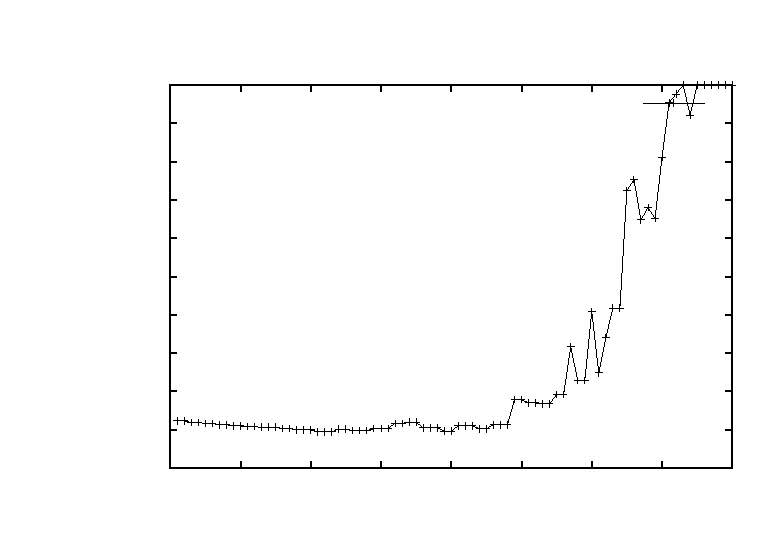
\includegraphics[width=10.0cm]{lebel3/ALPHA.eps}
  \caption{ALPHAの増加に伴う推移}
  \label{alpha}
 \end{center}
\end{figure}  
\subsubsection{考察}
出力結果を見ると,HIDDENの数値が結果に大きく影響することがわかる.HIDDENが低い場合,少し数値を増やすだけで値が大幅に更新されるが,30を超えた辺りから増加に転じた.このパラメータは増加させることで非常に学習に影響をおよぼすが,性能の向上には限界がある.しかし,値の刻み幅も1だけなのでまずことのパラメータを調整することにした.次にETAは数値を増やしていくことで次第に最小値へ近づくように変化するパラメータであることがわかった.値の影響は大きいが,刻み幅を狭くしてもそれほど結果に表れなかった.一方でALPHAは増やせば増やすほど収束までの時間がかかった.これは$\alpha$が学習の際にどれぐらい値を増やすか,という数値になっているため,精度は増すが学習に時間がかかるという結果になったことがわかる.
